%%%%%%%%%%%%
%
% $Autor: Wings $
% $Datum: 2019-03-05 08:03:15Z $
% $Pfad: Functions.tex $
% $Version: 4250 $
% !TeX spellcheck = en_GB/de_DE
% !TeX encoding = utf8
% !TeX root = manual 
% !TeX TXS-program:bibliography = txs:///biber
%
%%%%%%%%%%%%

\chapter{First Steps}

Once your environment is set up, follow these steps to start using the dataset and models:

\section{Setting Up the Project Locally}

Download or clone the project repository to your local machine.

\begin{enumerate}
	\item If using a GitHub repository, open a terminal, navigate to your desired directory, and run:
	\begin{verbatim}
		git clone https://github.com/your-repository-link.git
	\end{verbatim}
	
	\item If you do not use Git, you can manually download the project files as a ZIP archive from GitHub and extract them to your preferred folder.
\end{enumerate}

\section{Installing Dependencies}

Before running the application, ensure you have Python (version 3.9 or higher recommended) and pip installed. Then, install the required libraries:

\begin{verbatim}
	pip install -r requirements.txt
\end{verbatim}
\begin{figure}[h]
	\centering
	\fbox{\includegraphics[width=1.1\textwidth]{D:/BA_PROJECT/BA25-02-Time-Series/Manual/images/Intall requirements.png}}
	\caption{Installing the Required Python libraries}
\end{figure}


\section{Running the Application}

To launch the application, use the following command in your terminal from the project directory:

\begin{verbatim}
	streamlit run app.py
\end{verbatim}

This will open the application in your default web browser, where you can upload your data and generate predictions.

\begin{figure}[h]
	\centering
	\fbox{\includegraphics[width=1.1\textwidth]{D:/BA_PROJECT/BA25-02-Time-Series/Manual/images/Streamlit.png}}
	\caption{Streamlit Command}
\end{figure}




\section{Running the Preprocessing and Prediction Models}

Once you have installed the necessary libraries and set up the project, you can use the application to generate hurricane intensity predictions with the pre-trained ARIMA and LSTM models. Follow these steps:

\textbf{Step 1: Launch the Application}

Open a terminal, navigate to the project directory, and run the following command to start the Streamlit app:

\begin{verbatim}
	streamlit run app.py
\end{verbatim}

This will open the application in your default web browser.

\textbf{Step 2: Upload Your Data}

On the web interface, you will see an option to upload your hurricane dataset.

Ensure your data is formatted according to the required structure (date, time, location, wind speed, pressure, etc.).

Upload your file using the provided upload button.

\begin{figure}[h]
	\centering
	\fbox{\includegraphics[width=1.1\textwidth]{D:/BA_PROJECT/BA25-02-Time-Series/Manual/images/Upload.png}}
	\caption{Uploading the File}
\end{figure}


\textbf{Step 3: Generate Predictions}

Once your data is uploaded, the application will automatically use the pre-trained ARIMA and LSTM models to generate predictions.

The models have been pre-trained by the developer using optimal parameters and are stored in the \texttt{models/} folder. You do not need to set or adjust any parameters.

\textbf{Step 4: View and Download Results}

The predicted results will be displayed on the web interface.

You will also have the option to download the predictions as a CSV file for further analysis.

\textbf{Notes}

\textbf{No Training Required:} You do not need to train the models or set any parameters. All model training and parameter selection have been handled by the developer.

\textbf{Pre-trained Models:} The application uses models that have already been trained and saved. Your uploaded data is only used for generating predictions.

\textbf{Model Files:} The ARIMA and LSTM model files are stored in the \texttt{models/} directory and are loaded automatically by the application.

\begin{figure}[h]
	\centering
	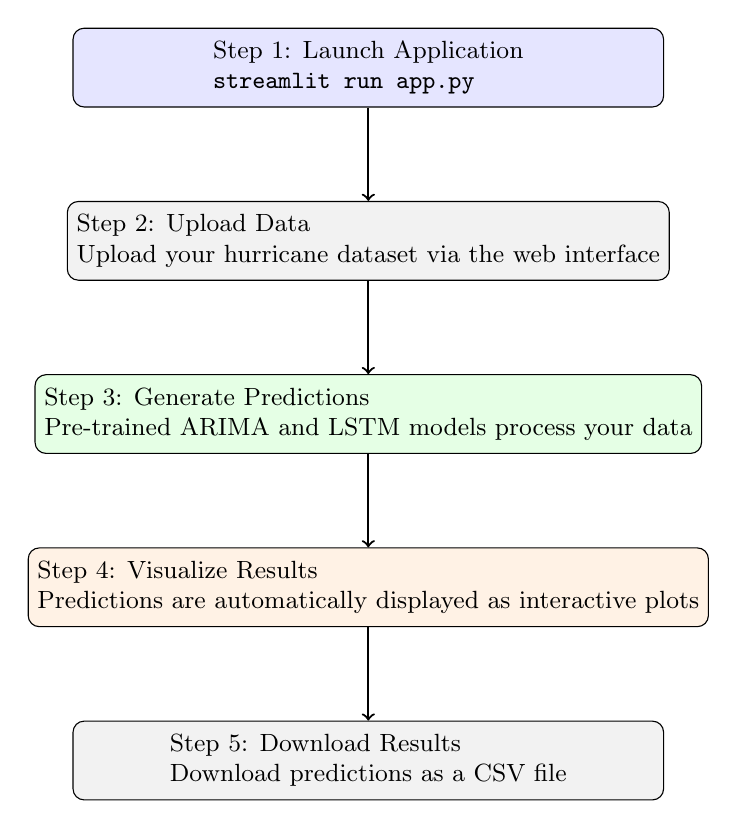
\begin{tikzpicture}[
		node distance=2.2cm,
		every node/.style={draw, rounded corners, minimum width=7.5cm, minimum height=1cm, align=left, font=\small}
		]
		% Steps
		\node[fill=blue!10] (launch) {Step 1: Launch Application\\\texttt{streamlit run app.py}};
		\node[below of=launch, fill=gray!10] (upload) {Step 2: Upload Data\\Upload your hurricane dataset via the web interface};
		\node[below of=upload, fill=green!10] (predict) {Step 3: Generate Predictions\\Pre-trained ARIMA and LSTM models process your data};
		\node[below of=predict, fill=orange!10] (visual) {Step 4: Visualize Results\\Predictions are automatically displayed as interactive plots};
		\node[below of=visual, fill=gray!10] (download) {Step 5: Download Results\\Download predictions as a CSV file};
		
		% Arrows
		\draw[->, thick] (launch) -- (upload);
		\draw[->, thick] (upload) -- (predict);
		\draw[->, thick] (predict) -- (visual);
		\draw[->, thick] (visual) -- (download);
	\end{tikzpicture}
	\caption{Workflow for Running Preprocessing, Prediction, and Visualization}
\end{figure}

\clearpage

\section{Visualizing the Predictions}

After you upload your data and predictions are generated, the results are automatically visualized within the Streamlit application. You will see interactive plots for both ARIMA and LSTM model predictions directly on the web interface.

No additional steps or code are required to display these visualizations. The app handles all plotting internally using Matplotlib and Streamlit's \texttt{st.pyplot()} function.

If you wish to save or further analyze the plots, you can use the download options provided in the app or take screenshots as needed.


